\documentclass[letterpaper]{article}

\usepackage[utf8]{inputenc}
\usepackage{amsmath}
\usepackage{listings}
\usepackage{hyperref}
\usepackage{graphicx}
\usepackage{comment}

\graphicspath{ {./images/} }

\title{A DSL for writing safer string manipulation functions in C}
\author{Michael Flanders}
\date{December 16, 2020}

%You can skip explaining the state of the art (i.e., how the problem is solved today).
%Instead, make sure to include a description of your language. Ideally,
%  you present a language tutorial using your previously selected examples. 
%When explaining your design, refer back to the architecture of DSL
%  implementations, similarly to how we asked you about the FFTW architecture
%  in the reading homework. 
%Please make your design description point to the relevant lines of your implementation.
%  Ideally, your doc will include links to the range of code in your github repo. 
%Please share the repo with the user rbodik. 
%Include the answers to the questions from the last slide.
%Please add the answer to the question "What knowledge or skill would have helped you
%  be more successful with the project."  The answers will help us in further upgrading
%  the course. 

\begin{document}
\maketitle

% Overview of project
% Overview of the sections

For this project, I built a DSL that prevents the common string and
integer related vulnerabilities and undefined behaviors in C programs.
The DSL is a small, restricted subset of C with some additional constructs
like $String$ types, range and subrange constraints, and bounded,
fold-style loops. By raising the abstraction level of strings and loops
and using the range constraints in typechecking and static analysis,
most of the common string vulnerabilities can be eliminated.

This report provides an analysis of the problem domain, a description
of the DSL, a breakdown of the design and design decisions made, and
a discussion of the project.

\section{Domain analysis}

I built the DSL as a development aid for new or moderately experienced
C developers. These developers would be writing some C application
that needs to handle user input, and that user input is often a string.
The input validation, sanitization, and processing functions would be
written in the DSL, compiled to a header file, and then imported to
the project to help provide a stronger outer shell.

These security guarantees do have a cost since the performance of the
generated C code cannot compare to the performance that an experienced
C developer might be able to achieve. However, I would argue that even
using the DSL only on validation, sanitization, and pre-processing code would
provide a lot of security benefits while only having a slight performance
impact (since most of the program logic is probably not contained in these
routines).

\subsection{A motivating example}

There are many codebases that could benefit from having their input processing
code rewritten in the DSL, but here I provide only one such example where the
DSL beats static analyzers, symbolic execution, and fuzzers. I do not
provide code here since I think distributing decompiled, closed-source code
is not very legal, but the example is from a vulnerability I found in Netgear
routers last year: https://www.zerodayinitiative.com/advisories/ZDI-19-866/.

The code snippet below shows a function from the mini\_httpd
HTTP server that decodes HTML-Url encoded strings. This
same code is used in thttpd which powers sites such as
images.paypal.com, garfield.com, drudgereport.com, and
the official website of the Sovereign Principality of Sealand.

Another notable user of mini\_httpd is Netgear. Earlier
models of Netgear routers (pre-2018), use a modified version of mini\_httpd
with modifications to the decoding and sanitization functions such as
the one shown below. These modifications make connecting to the router
from the Netgear phone app simpler, but also introduce a severe vulnerability
that allows networks guests to execute arbitrary code on the router
as an administrator.


%\begin{figure}
%  \centering
  \begin{lstlisting}
  static void
  strdecode( char* to, char* from )
  {
    for ( ; *from != '\0'; ++to, ++from )
    {
      if ( from[0] == '%' && isxdigit( from[1] ) && isxdigit( from[2] ) )
      {
	*to = hexit( from[1] ) * 16 + hexit( from[2] );
	from += 2;
      }
      else
      *to = *from;
    }
    *to = '\0';
  }
  \end{lstlisting}
%  \caption{Code snippet from mini\_httpd}
%  \label{fig:minihttpd}
%\end{figure}

This is a case where the DSL would shine; static analyzers, symbolic
execution, and fuzzing would all miss the vulnerability. The vulnerability
is caused by an incorrect implementation of a check for contained substrings
and bad pointer arithmetic. However, there is no undefined behaviour or
out-of-bounds accesses, so static analyzers and tools like KLEE or CBMC
will not warn. The strings needed to trigger the vulnerability are also
very complex; the vulnerability requires providing valid URL's that the
server transforms into an exploit/payload during sanitization and validation.
By providing a very carefully crafted URL, an attacker can trick the server
into inserting a null-byte within a string buffer (this turns one string into
two and is called a poison null-byte vulnerability), performing validity checks on the
second string, and then using the first string. Complex dependencies on
network connections and filesystem further complicate the situation for fuzzers.

Writing the validation and decoding functions in the DSL would have avoided
this vulnerability. Even though there is no guarantee on functional correctness
of programs written in the DSL, the high-level string functions remove the
need to worry about null bytes and terminators, so this vulnerability could not
even have been written. In other words, the \textit{pre-provided} string functions in the DSL
should always compile to safe and functionally correct C code which is enough
in this case.

\section{Language description}

% Overview
% Paradigm, immutability, boundedness
% Language constructs, operators
% Ranges, subranges
% For loops

\section{Design and decisions}

\begin{figure}[h]
  \centering
  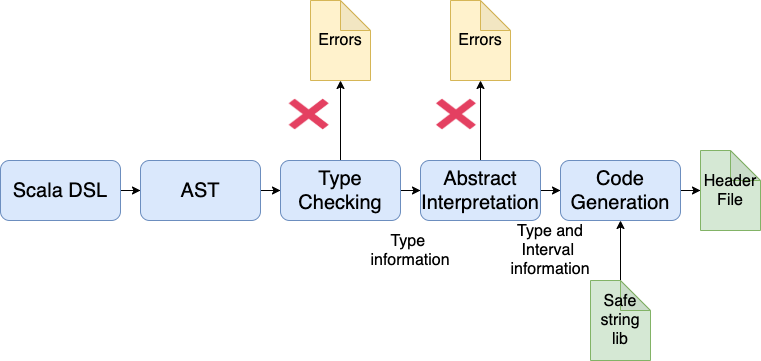
\includegraphics[width=\textwidth]{architecture.png}
  \caption{Diagram of the compiler pipeline}
  \label{fig:pipeline}
\end{figure}

\begin{figure}[h]
  \centering
  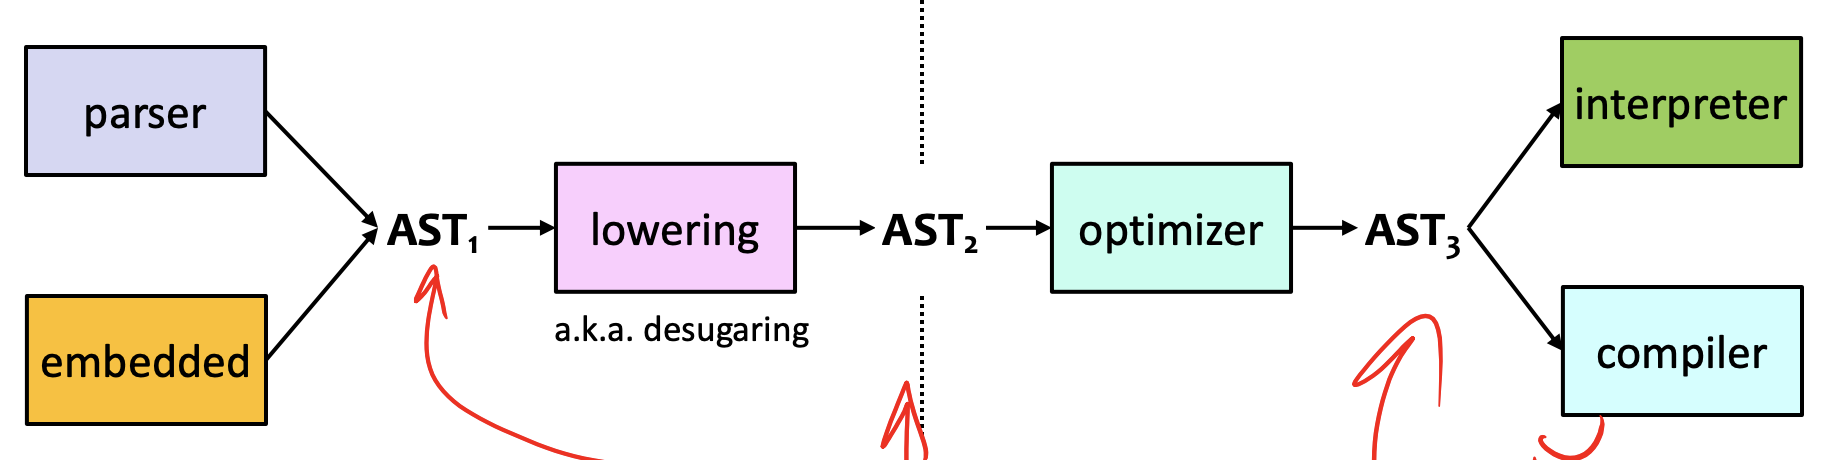
\includegraphics[width=\textwidth]{modern-compiler-pipeline.png}
  \caption{Diagram of the compiler pipeline. (Screenshot from the marked up lecture slides)}
  \label{fig:mdnpipeline}
\end{figure}

% Overview
% Lexer/parser vs fluent-syntax/call-chaining
% Typechecker
%  the basics and some of the other checks:
%   no recursion
%   ranges well formed (lower bound <=  upper bound)
%  monadic, pretty proud of this. Lots of Option,Either mixed, wished it was cleaner still
% Abstract interpreter
%  abstract domain is intervals
%  didn't finish, couldn't get 
%  everything is bounded, all loops end => widening and narrowing are optimizations
%   not necessities, so easier to just build abs int, act like normal interpreter and
%   just ride loops out
%  vs symbolic execution
%   ended up seeming like more work getting the integer semantics symbolic but
%   i think it would've ended up just as precise but a little slower
% Code generation
%  Didn't finish this, couldn't get:
%    most of the string functions written
%    freeing of complicated data
%     2 solutions, copy/dupe all strings from iters or some kind of analysis
%  the safe string library
%    static inlined
%    could get the code gen to just write one C function but it ended up looking messy,
%     developers might not trust it

\section{Discussion}

% Answer the questions from the last slide (of the template?)
%  What are you proud of? A neat trick in the design or implementation
%    of your language.
%
%  Mistakes describe a mistak you made, e.g., a construct you think will confuse programmers
%
%  What we would do differently
%    Give the lessons you learnt in this project, if you have to start again, what would you do differently?
%
% "What knowledge or skill would have helped you be more successful in the project?"
%
%   Wish we got some deeper monadic/parametrized interpreter coding homeworks. I did the
%   all of the monads for functional programming and essence of fp examples, but they only
%   touched on one monad at a time and really simple semantics. I ended up only really underst
%   standing monad transformers and free monads 1-2 days before the final presentation, so I
%   wish I knew more about engineering an interpreter so I could've used this. Contrast w/
%   FFTW. example is checkStmt for For in typechecker
%   

\end{document}
